\documentclass[a4paper]{article}

\usepackage[dutch]{babel}
\usepackage{fullpage}
\usepackage{graphicx}
\usepackage{url}
\usepackage{wrapfig}
\usepackage[pdftex]{bookmark}

\newcommand{\casam}{C.A.S.A.M. }
\newcommand{\casamproject}{C.A.S.A.M.-pro\-ject }


\title{\casamproject Ori\"{e}ntatieverslag}
\author{S.E.F. van Berkel \and B. Bijl \and J.Y.T. den Hollander \and S. Rabbelier \and B.M.W. Sedee \and N.N. Smit}

\begin{document}

\begin{titlepage}

\maketitle

\thispagestyle{empty}

\end{titlepage}

\setcounter{page}{2}
\setcounter{tocdepth}{2}

\tableofcontents

\newpage

\noindent

\section{Inleiding}
\label{inleiding}


%\section{Projectbeschrijving}
\label{Projectbeschrijving}
 screw deze shit

\section{Medische aspecten}
\label{Medische aspecten}


Om een brug te slaan tussen de kennis van de medici en de technici is het voor de technici van belang om te beschikken over een basale kennis van de relevante anatomie van het menselijk lichaam en de begrippen die gebruikt worden. We hebben ons verdiept in de veelgebruikte basistermen en de relevante anatomie van het been. In de opdracht werd een onderzoek als voorbeeld gebruikt betreffende de venen en zenuwen van het onderbeen. Het ging hierbij om lasertherapie behandeling van spataderen (varices). Varices ontstaan als de venenkleppen niet meer naar behoren functioneren en het bloed niet meer goed terug naar het hart wordt geleid. De vraagstelling van het onderzoek is hierbij, wat zijn de veilige gebieden om de laserbehandeling uit te voeren, oftewel waar ligt de nabijgegelegen zenuw ver genoeg van de vene af? Met dit onderzoek in het achterhoofd hebben we de relevante anatomische kennis erbij gezocht.
De onderstaande kennis komt uit de Atlas an de Anatomie van Sesam.\cite{sesam}

\subsection{Anatomie basisterminologie}

Voor het aangeven van gebieden in het lichaam worden in de medische wetenschap bepaalde basisbegrippen gebruikt. Allereerst kan het menselijk lichaam opgedeeld worden in de hoofdgebieden. 
Zo is er de stam (truncus) en de bovenste en onderste ledematen (extremiteiten). 
De stam bestaat uit het hoofd (caput), de hals (collum) en de romp. 
De romp zelf bestaat uit de borst (thorax), buik (abdomen) en bekken (pelvis). 
De grens tussen truncus en de extremiteiten bevinden zich aan de bovenzijde bij de schoudergordel en aan de onderzijde bij de bekkengordel. 
Vervolgens zijn er vlakken beschreven die een doorsnede van het menselijk lichaam beschrijven. Deze lopen door de drie hoofdassen van het lichaam. Allereerst is er de verticale of longitudinale as. Dit is de lengte-as van het lichaam. Ten tweede is er de transversale of horizontale as. Deze as staat loodrecht op de verticale as en loopt van links naar rechts door het lichaam. De derde as is de saggitale as. Deze as staat loodrecht op de eerste twee assen en loopt van achteren naar voren door het lichaam. 

Op basis van de eerdergenoemde assen zijn vlakken door het lichaam te defini\"{e}ren:
\begin{itemize}
	\item Mediaan of mediaan-saggitaal vlak: door lengte- en saggitale as
	\item Saggitaal of paramediaan vlak: evenwijdig aan mediaan vlak
	\item Frontaal of coronaal vlak: door transversale assen, loodrecht op mediaan-saggitaal vlak
	\item Transversale vlakken: loodrecht op mediaan vlak en een frontaal vlak
\end{itemize}

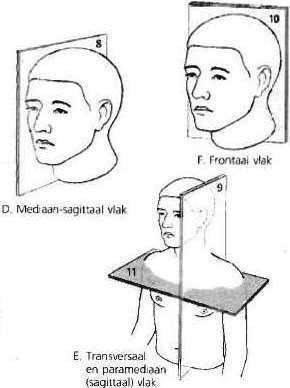
\includegraphics[width=0.9\textwidth]{sesam}

Om specifiekere gebieden aan te geven worden er een aantal termen gebruikt om een richting te omschrijven, hieronder een kort overzicht:
\begin{itemize}
	\item Craniaal: richting de schedel
	\item Superior/inferior: naar boven/naar beneden
	\item Mediaal/lateraal: naar het midden/van het midden af
	\item Centraal (profundus)/perifeer (superficialis): naar het inwendige/naar het oppervlakte
	\item Anterior/posterior: naar voren/naar achteren
	\item Proximaal/distaal: naar de bevestiging van de ledematen/ervan af
	\item Tibiaal/fibulair: naar het scheenbeen/naar het kuitbeen
	\item plantair : naar de voetzool toe
\end{itemize}

\subsection{Anatomie van het been}

Voor het begrip van de anatomie van het been bekijken we vervolgens de belangrijkste bot- vaat- en zenuwstructuren. 
Het gaat te ver om hier een uitgebreide beschrijving van te geven, wederom is slechts basiskennis benodigd. Wat betreft de botstructuren is er allereerst het bovenbeen (femur). De femur vormt de verbinding tussen de bekkengordel en de knie. Vervolgens is er de knieschijf (pattella) die het kniegewricht beschermd. In het onderbeen zijn het scheenbeen (tibia) en het kuitbeen (fibula) te vinden, deze vormen de verbinding tussen de knie en de enkel. In de voet bevinden zich vele botten, waarvan voor een ander onderzoek dat we gezien hebben het hielbeen (calcaneus) het meest relevant is. Belangrijke bony landmarks\footnote{landmarks die voortkomen uit de anatomie van het menselijk lichaam en voelbaar zijn vanaf de buitenkant} voor het onderbeen zijn onder andere de mediale en laterale malleolus. De mediale malleolus bevind zich aan de binnenzijde van de enkel en is een onderdeel van de tibia. De laterale malleolus bevindt zich aan de buitenzijde van de enkel en is een onderdeel van de fibula.

Wat betreft de vaatstructuren zijn er arteri\"{e}n en venen te onderscheiden. De vaatstructuren relevant voor het voorbeeldonderzoek bevinden zich in het onderbeen, het is met name de Vena Saphena Parva (VSP). Deze ontstaat aan de laterale voetrand en trekt door naar de Vena Poplitea, die zich bij de knie bevindt. De nabijgelegen zenuw die relevant is is de surale zenuw (Nervus Suralis) welke een vertakking is van de Nervus Tibialis.




\section{Image Processing Technieken}
\label{Image Processing Technieken}
In dit hoofdstuk gaan we in op de theorie achter de gebruikte Image Processing technieken. 
Allereerst beginnen we met een beschrijving van het Point Distribution Model, dit doen we aan de hand van Generalised Procrustes Analysis en Principal Component Analysis. 
Tot slot bespreken we kort de theorie achter de Thin Plate Spline transformatie. 

\subsection{Point Distribution Model}
Het Point Distribution Model is een model dat de gemiddelde vorm en modes van variatie kan weergeven.\cite{PDM} 
Een vorm is hierbij een vorm alles wat overblijft als alle locatie, schaling en rotatie effecten eruit gefilterd zijn.\cite{gpa}
Om een vorm te beschrijven aan de hand van een set van voorbeelden is er een manier nodig om de vorm te defini\"{e}ren. 
Dit is mogelijk door de expert met landmarks belangrijke punten in de vorm aan te geven. 
Een landmark is in dit geval een punt dat duidelijk herkenbaar moet zijn in elke foto. 
Dit kan een bony landmark (komt voort uit de anatomie van de mens) of een zelf gekozen landmark. Een voorbeeld van een landmark bij een foto van de hand kan het topje van de duim zijn. 
Gegeven een set van \textit{n} landmarks aangegeven in een aantal voorbeelden van een vorm kan er een statistisch shape model worden opgesteld. 
Om dit te bereiken moeten de foto's eerst in eenzelfde co\"{o}rdinatenframe worden gezet. Dit wordt gedaan met Generalized Procrustes Analysis.

\subsubsection{Generalised Procrustes Analysis}
Procrustus Analysis kan worden gebruikt om 2 sets van landmarks uit te lijnen. Generalised Proctrustes Analysis echter kan worden gebruikt om \textit{k} sets van landmarks met elkaar uit te lijnen. 
Het transleert, roteert en schaalt (eventueel) elke vorm door de som van de gekwadrateerde afstanden tot het gemiddelde te minimaliseren. 

Het algoritme van Generalised Procrustus Analysis werkt als volgt\cite{gpa}:
\begin{enumerate}
	\item Selecteer 1 vorm als tijdelijk gemiddelde vorm
	\item Lijn de overige shapes uit met deze vorm:
	\begin{itemize}
		\item Bereken het centroid van elke vorm.
		\item Lijn alle vormen uit naar de oorsprong.
		\item Normaliseer de grootte van de centroid van elke vorm.
		\item Roteer de vorm om uit te lijnen met het nieuwste geschatte gemiddelde.
	\end{itemize}
	\item Bereken het nieuwe geschatte gemiddelde uit de uitgelijnde vormen.
	\item Als het geschatte gemiddelde uit stap 2 en 3 anders zijn, ga dan naar 2 terug. Als dit niet zo is is het ware gemiddelde gevonden.
\end{enumerate}

Elke vorm kan nu gerepresenteerd worden als een \textit{2n} element vector:\
$x = (x_{1},...,x_{n},y_{1},...,y_{n})$ 

De uitgelijnde trainingsets vormen nu een wolk in de \textit{2n} dimensionale ruimte. Door Principal Component Analysis uit te voeren kunnen de hoofdassen van de wolk worden berekend.

\subsubsection{Principal Component Analysis}

Principal Component Analysis (PCA) is een manier om patronen in data te herkennen, en de overeenkomsten en verschillen binnen de dataset weer te geven.\cite{pca}
Als je van alle vectoren de covariantiematrix \textit{S} uitrekent en hierop eigen-analyse uitvoert wordt de vorm van de \textit{m x n}-dimensionale puntenwolk een gewogen som van orthogonale vectoren. Hierin zijn de gewichten de eigenwaarden \lambda en de 'assen' die de ruimte opspannen de eigenvectoren \textit{p}. 
De eigenvectoren waarbij de grootste eigenwaarden horen staan hierbij voor de grootste variaties in de dataset. 
De eigenvector met de hoogste eigenwaarde is de Principal Component, de meest significante relatie tussen de dimensies van de data. 
De overige eigenvectoren p representeren de andere principal directions. Elk punt op het oppervlakte van het object kan nu gerepresenteerd worden als een lineaire combinatie van p toegevoegd aan de centroid of het gemiddelde van de vorm.

Het algoritme:

    * Verkrijg de datapunten
    * Trek er het gemiddelde van af
    * Bereken de covariantie matrix
    * Bereken de eigenvectoren en waarden
    * Choosing and forming feature vector
    * Derive new dataset
    * Get old data back 
    
    
We use Principal Component Analysis (PCA) to pick out the main axes of the cloud, and model only the first few, which account for the majority of the variation.
The shape model is then

$x = x_mean + Pb$

where $x_mean$ is the mean of the aligned training examples, P is a 2n x t matrix whose columns are unit vectors along the principal axes of the cloud, and b is a t element vector of shape parameters.

(This model has been dubbed a "Point Distribution Model" (PDM), but has little to do with the Point Distribution in statistics)

By varying the shape parameters within limits learnt from the training set, we can generate new examples.

Such models are used in the Active Shape Model framework to locate new examples in new images.
Hand Example

Consider the outline of a hand, represented by 72 labelled points.
Here are some examples from a training set:

By varying the first three parameters of the shape vector, b, one at a time, we can demonstrate some of the modes of variation allowed by the model:

(Each row obtained by varying on parameter and fixing others at zero)
Face Example

Here represent the shape of the facial structures with 68 points

The first mode of shape variation of a training set containing many different view points tends to represent rotation of the head.
Brain Structure Example

We can represent the outline of several brain structures in a single model.
For instance, here is an example from a labelled brain MR image

By varying the first two parameters of the shape vector, b, one at a time, we can demonstrate some of the modes of variation allowed by the model:

Varying the most significant parameter.

Varying the second most significant parameter.
More Complex Shape Models
In some situations, the gaussian approximation is simplistic, as the pdf for the shapes is significantly non-gaussian. This can arise if sub-parts of the modelled object rotate, leading to curved clouds of training points in the shape space. Several methods have been used to model such clouds. Polynomial approximations (Sozou et al), neural-net formulations (Sozou et al), and polar co-ordinates (Heap en Hogg) have all been tried. The most recent approach is to treat the cloud as a sample from a pdf, use kernel methods to estimate the pdf, and then to approximate this pdf using a mixture of gaussians. The Expectation Maximisation algorithm is used to fit the mixture to the data. To simplify the calculations, PCA is used to determine a low dimensional sub-space containing most of the variation, before the kernel method is applied. In effect, we use the same model as above, but determine stricter limits on the allowed values of the shape parameters b, modelling their distribution with a mixture of gaussians instead of a single gaussian. The allowed values are those for which the pdf is above a threshold, which can be determined using monte-carlo methods from the mixture .


\subsection{Thin Plate Spline Transform}
%TODO: Noeska, get started on this


\section{Software}
\label{Software}
In dit hoofdstuk bespreken we de softwaretechnologi/"{e}n die we gaan gebruiken om de applicatie te maken. 
We beginnen met de basis van de applicatie door eerst de IDE, Python en Django te bespreken. 
Hierna bespreken we de 2 gebruikte bibliotheken, VTK en PIL. 
Tot slot bespreken we kort JavaScript en Flash.

\subsection{Integrated Development Environment (IDE): Eclipse}
%TODO: Write something nice about Eclipse and PyDev? Any volunteers?

\subsection{Python}
%TODO: Sverre, go wild!

\subsection{Django}
%TODO: Sverre, go wild! Once again!

\subsection{Visualisation Toolkit (VTK)}
Voor het implementeren van de benodigde Image Processing Technieken maken we gebruik van de Visualisation Toolkit (VTK)\cite{vtk}. 
VTK is een open source toolkit voor 3D graphics. 
In ons geval zetten we de toolkit in voor 2D graphics. 
VTK bestaat uit een C++ class bibliotheek en onder andere een Python interface laag.\cite{vtk2} 
Er zitten uitgebreide mogelijkheden in op het gebied van Image Processing en visualisatie.
In de VTK zitten de benodigde filters om Generalized Procrustes Analysis en Principal Component Analysis uit te voeren. 
Verder bevat de toolkit een implementatie van de Thin Plate Spline transformatie. 
Door de z-co\"{o}rdinaten op 0 te zetten kan VTK in de 2D ruimte worden gebruikt. 

\subsection{Python Imaging Library (PIL)}
Om de wat simpelere Image Processing technieken te implementeren maken we gebruik van de Python Imaging Library (PIL)\cite{pil}. 
Er is een handbook beschikbaar waarin de functionaliteiten besproken worden.\cite{pilhandbook} 
Dit kan onder andere ingezet worden voor het resizen van images, puntoperaties, filtering, colour space conversies, rotatie en transformaties. 

\subsection{JavaScript}
Om een mooie en gebruiksvriendelijke user-interface te krijgen, gaan wij gebruik maken van JavaScript.
Hiervoor zijn er een aantal bibliotheken beschikbaar die ons gaan helpen (Scriptaculous\cite{scriptaculous} en Prototype\cite{prototype}).
Prototype gaan we onder andere gebruiken vanwege de mooie mogelijkheden om met AJaX om te gaan, en de handige manieren om objecten aan te maken.
De Scriptaculous bibliotheek biedt ons verschillende mogelijkheden voor visuele toepassingen binnen een website, zoals sliders en draggables

\subsection{Flash}
%TODO: Bastiaan, your expertise, show us it.
%messing up the order ^^

\newpage
\bibliographystyle{plain}
\bibliography{Orientatie}

\end{document}

